\chapter{نحوه‌ی استقرار مدل و تکنولوژی‌های استفاده‌شده}

در این بخش ابتدا به طریقه‌ی استقرار\LTRfootnote{Deploy} مدل یادگیری ماشین سیستم پیاده‌شده اشاره می‌کنیم و در قسمت‌های بعد تکنولوژی‌های اصلی دخیل در توسعه این دستگاه را به طور دقیق مورد بررسی قرار می‌دهیم. شایان ذکر است که مدل یادگیری ماشین به صورت یک سرویس مجزا به کارگزار\LTRfootnote{Server} جمع‌آوری اطلاعات لرزش گره‌ها که در یک پروژه‌ی مجزا در راستای پروژه‌ی کنونی توسعه یافته است، اضافه شده است.

\section{نحوه‌ی استقرار مدل یادگیری ماشین}
 روش‌های مختلفی برای استقرار و استفاده از مدل‌های یادگیری هوش مصنوعی مورد استفاده قرار می‌گیرند که از بین اینها چهار روش نشان داده‌ شده در \cref{fig:ml_model_deployments} مرسوم‌تر هستند\cite{kaggleMLdeployments}:

\begin{figure}[!h]
\centerline{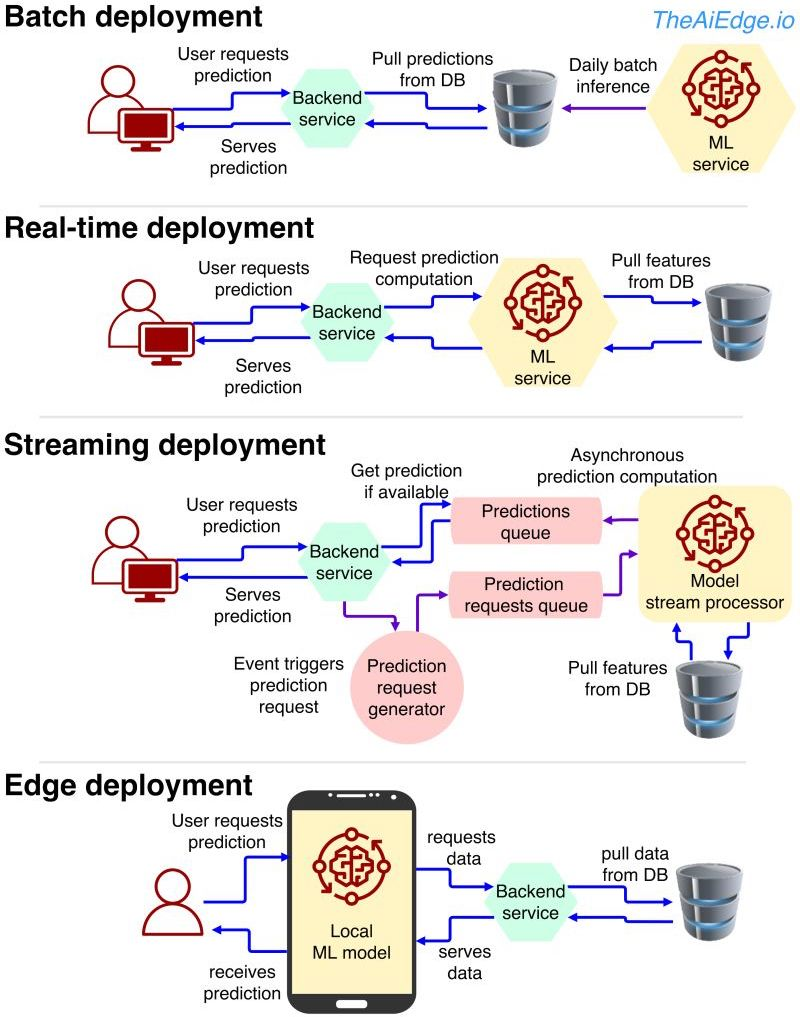
\includegraphics[width=.5\textwidth]{ml_model_deployments.png}}
\caption{انواع روش‌های استقرار مدل‌های یادگیری ماشین}
\label{fig:ml_model_deployments}
\end{figure}

\begin{itemize}

\item \textbf{پیاده‌سازی دسته‌ای\LTRfootnote{Batch Deployment}}: پیش‌بینی‌ها به فاصله‌های زمانی مشخص محاسبه می‌شوند و پیش‌بینی‌های حاصل در پایگاه داده ذخیره می‌شوند و به راحتی می‌توان آنها را در صورت نیاز بازیابی کرد. با این حال، نمی‌توان از داده‌های بروزتر استفاده کرد و پیش‌بینی‌ها می‌توانند به سرعت منسوخ شوند\cite{singh2021deploy, pacheco2018towards}.

\item \textbf{پیاده‌سازی بی‌درنگ\LTRfootnote{Real-Time Deployment}}: در این نوع از استقرار، درخواست کاربر برای گرفتن جدید‌ترین پیش‌بینی‌ها به عنوان یک راه‌انداز\LTRfootnote{Trigger} توسط رابط برنامه‌نویسی\LTRfootnote{Application Programming Interface (API)} اچ‌تی‌تی‌پی\LTRfootnote{Hypertext Transfer Protocol (HTTP)} به کارگزار ارسال می‌شود. سپس سرویس یادگیری ماشین که به عنوان افزونه‌ای در سمت کارگزار توسعه یافته است، شروع به کار می‌کند و جدیدترین نتایج پیش‌بینی را تولید و ذخیره می‌کند و به سمت کاربر به عنوان نتیجه ارسال می‌کند. مشکل اصلی این روش قرارگیری مدل یادگیری ماشین، کند بودن روند یادگیری و پیش‌بینی است که منجر به منتظر ماندن کاربر می‌گردد. می‌توان با بهره‌گیری از فرآیند\LTRfootnote{Process}‌های چندریسمانی\LTRfootnote{Multi-Threaded} برای دریافت درخواست‌های کاربر و انجام مرحله‌ی یادگیری و پیش‌بینی مدل، تا حد زیادی این مشکل را برطرف کرد\cite{singh2021deploy, pacheco2018towards}.

\item \textbf{پیاده‌سازی جریانی\LTRfootnote{Streaming Deployment}}: این امکان را می‌دهد تا فرآیند ناهمزمان‌\LTRfootnote{Asynchronous}تری ایجاد شود. یک رویداد می‌تواند شروع فرآیند استنتاج را فراهم کند. این فرآیند در صف یک واسط پیام\LTRfootnote{Message Broker} مانند کافکا\LTRfootnote{Apache Kafka} قرار داده می‌شود و مدل یادگیری ماشینی در هنگام آماده شدن برای انجام درخواست، آن را انجام می‌دهد. این کار به سرویس پشتیبانی فرصت می‌دهد و با فرآیند صف بهینه، قدرت محاسباتی بسیاری را صرفه‌جویی می‌کند. پیش‌بینی‌های حاصل شده نیز در صف قرار گرفته و در صورت نیاز توسط سرویس‌های پشتیبانی مصرف می‌شوند. از مزیت‌های این روش نسبت به روش بی‌درنگ، می‌توان به کم‌شدن تاخیر پاسخ‌دهی به کاربران اشاره کرد\cite{singh2021deploy, pacheco2018towards}.

\item \textbf{پیاده‌سازی لبه‌ای\LTRfootnote{Edge Deployment}}: در این روش استقرار، مدل مستقیماً بر روی کلاینت نصب می‌شود، مانند مرورگر وب، یک تلفن همراه یا محصولات اینترنت اشیاء. این کار باعث رسیدن به سریع‌ترین استنتاج می‌شود، اما معمولاً مدل‌ها باید به اندازه کافی کوچک باشند تا بتوانند در سخت‌افزارهای کوچکتر نصب شوند\cite{kaggleMLdeployments}.

\end{itemize}

بدلیل اینکه گره‌های موجود در شبکه‌ی اشیاء دارای توان پردازشی محدود هستند و اینکه ماهیت مدل هوش‌ مصنوعی مربوط به حوزه‌ی کاری پیش‌بینی عمر دستگاه‌ها بدین‌گونه است که حتما باید از داده‌های مربوط به همه‌ی گره‌های موجود استفاده کرد، با توجه به گزینه‌های مطرح‌شده برای استقرار مدل هوش مصنوعی توسعه‌داده شده و همچنین مزایا و معایب هر کدام، از روش استقرار بی‌درنگ برای ارائه و بکارگیری مدل هوش مصنوعی در این پروژه استفاده شده است. به طور دقیقتر، مدل هوش مصنوعی به عنوان یک سرویس اضافی برای کارگزار اصلی توسعه‌ داده‌شده در پروژه‌ی مرتبط 
به این پروژه تعبیه شده است. در بخش‌های بعد، به زبان برنامه‌نویسی و چارچوب‌\LTRfootnote{Framework}های بکارگرفته شده برای آماده کردن این سرویس اشاره خواهیم کرد. 

\section{‌‌زبان برنامه‌نویسی}
برای انتخاب زبان برنامه‌نویسی مناسب برای توسعه مدل یادگیری ماشین شرح‌داده شده، باید معیارهای متفاوتی را در نظر گرفت. برای این منظور زبان پایتون\LTRfootnote{\href{https://docs.python.org/3/}{Python}} را برگزیدیم. مواردی همچون داشتن چارچوب‌ها و کتابخانه‌های قدرتمند یادگیری ماشین، توسعه‌ی آسان و سریع و محبوبیت بالا از دلایل اصلی انتخاب پایتون به عنوان زبان اصلی برای توسعه‌ی سرویس یادگیری ماشین می‌باشد. همچنین شایان ذکر است که چون کارگزار اصلی جمع‌آوری اطلاعات لرزش به زبان پایتون نوشته شده است، استفاده از این زبان برای توسعه مدل یادگیری ماشین، باعث بهبود توسعه‌پذیری نیز می‌گردد. 

\subsection{زبان برنامه‌نویسی پایتون}
